\documentclass[11pt]{article}
\usepackage[margin=0.9in]{geometry}
\usepackage[T1]{fontenc}
\IfFileExists{lmodern.sty}{\usepackage{lmodern}}{\usepackage{mathptmx}}
\usepackage{amsmath,amssymb}
\usepackage{booktabs,tabularx,array,multirow}
\usepackage{enumitem}
\usepackage{titlesec}
\usepackage{xcolor}
\usepackage{graphicx}
\usepackage{caption}
\usepackage{float}
\usepackage[hidelinks]{hyperref}
\usepackage{xurl}
\graphicspath{{../results/figures/}}

\titleformat{\section}{\large\bfseries}{\thesection.}{0.5em}{}
\titleformat{\subsection}{\normalsize\bfseries}{\thesubsection}{0.5em}{}
\titlespacing*{\section}{0pt}{9pt}{3pt}
\titlespacing*{\subsection}{0pt}{5pt}{2pt}
\setlist{itemsep=1pt,topsep=2pt}
\setlength{\parskip}{4pt}
\setlength{\parindent}{0pt}
\renewcommand{\arraystretch}{1.12}
\newcolumntype{L}{>{\raggedright\arraybackslash}X}
\newcolumntype{R}{>{\raggedleft\arraybackslash}X}
\captionsetup{font=small,labelfont=bf,skip=3pt}
\emergencystretch=2em
\renewcommand{\topfraction}{0.9}\renewcommand{\textfraction}{0.08}\renewcommand{\floatpagefraction}{0.8}

\newcommand{\repo}{\url{https://github.com/Sathish049/cyb599-threshold-ckks}}

\begin{document}
\sloppy

\begin{center}
{\Large\bfseries Implementation and Evaluation: Threshold CKKS for\\[2pt] Privacy-Preserving Multi-Site Health Analytics}\\[7pt]
CYB 599 Graduate Project -- Part 3: Implementation \& Evaluation\\[3pt]
Sathish Reddy Pidugu \quad$\cdot$\quad \href{mailto:sp3754@nau.edu}{sp3754@nau.edu} \quad$\cdot$\quad November 16, 2026\\[3pt]
Code: \repo
\end{center}

\section{Summary}

I implemented the Part~2 protocol in Python on OpenFHE~[9] and evaluated it on a synthetic three-hospital cohort (15{,}000 patients, 7 features, 19.1\% readmission). Every party holds one share of an $n$-out-of-$n$ CKKS key. An untrusted server aggregates encrypted statistics and runs 27 iterations of encrypted gradient descent, refreshing ciphertexts with interactive multiparty bootstrapping~[4]. The analyst decrypts only the final result, from noise-flooded partial decryptions. The headline results:
\begin{itemize}
  \item \textbf{Correct.} 9 of 9 automated tests pass. On the Part~2 parameter set, encrypted coefficients match plaintext gradient descent to $6.0\times10^{-7}$ (20.7 bits), and pooled moments to a relative error of $2.4\times10^{-7}$.
  \item \textbf{Fast enough.} Private regression takes 5.2~s of online compute, against 3.4~ms for the non-private baseline (about 1{,}500$\times$ slower). Every Part~2 time budget is met with at least a 10$\times$ margin.
  \item \textbf{Three parameter sets} ($N=2^{14},2^{15},2^{16}$) show a three-way trade-off between interaction, precision and resources. The deep set avoids refreshes but is 5$\times$ slower and needs 3.9~GB of RAM.
  \item \textbf{One design flaw found and fixed.} Part~2's regression on publicly scaled features is still 97\% away from the exact coefficients after 27 iterations. A standardization round fixes this, at the cost of releasing 14 extra statistics (Section~\ref{sec:conv}).
\end{itemize}

\section{Implementation}\label{sec:impl}

\textbf{Structure.} The repository (\repo) has four modules: \texttt{params.py} (parameter sets), \texttt{data.py} (synthetic cohort and the public clipping bounds), \texttt{baseline.py} (the non-private reference) and \texttt{protocol.py} (sites, server and analyst). Table~\ref{tab:map} maps each Part~2 phase to the code.

\begin{table}[H]
\centering\small
\caption{Part~2 protocol phases and where they are implemented.}\label{tab:map}
\begin{tabularx}{\textwidth}{@{}p{4.1cm}p{4.4cm}L@{}}
\toprule
\textbf{Part 2 phase} & \textbf{Code (\texttt{protocol.py})} & \textbf{OpenFHE primitives} \\
\midrule
1. Collective key generation & \texttt{ThresholdCKKS.keygen} & \texttt{MultipartyKeyGen}, \texttt{MultiKeySwitchGen}, \texttt{MultiMultEvalKey}, \texttt{MultiEvalAtIndexKeyGen} \\
2. Local encryption & \texttt{run\_mode\_a}, \texttt{encrypt\_regression\_inputs} & diagonal packing~[8], \texttt{Encrypt} \\
3. Server evaluation (Algorithm 1) & \texttt{run\_regression}, \texttt{\_rotations} & \texttt{EvalMultNoRelin}, \texttt{Relinearize}, \texttt{Rescale}, \texttt{EvalFastRotation} \\
4. Collective refresh & \texttt{refresh} & \texttt{IntMPBootDecrypt/Add/Encrypt} \\
5. Threshold decryption, release & \texttt{decrypt}, \texttt{round\_sig} & \texttt{MultipartyDecryptLead/Main/Fusion} \\
Integrity layer I1 & \texttt{verify\_transcript} & SHA-256 over serialized ciphertexts \\
\bottomrule
\end{tabularx}
\end{table}

The protocol runs in two rounds. In round~1 (Mode~A) each site encrypts 17 moments of its publicly scaled data, and the analyst releases $N$, 7 feature means and 7 standard deviations, rounded to 4 significant digits. In round~2 (Mode~B) sites standardize their features with those statistics and encrypt the 8 diagonals of $-\tfrac{\eta}{N}X_j^\top X_j$ and the vector $\tfrac{\eta}{N}X_j^\top y_j$. The server runs $\beta_{t+1}=M\beta_t+c$ with one ciphertext level per iteration and refreshes every $L-2$ iterations. Only the 8 coefficients are decrypted.

\textbf{Changes from the Part~2 design.} Implementation surfaced four deviations, each backed by a measurement:
\begin{enumerate}[label=\textbf{C\arabic*.},leftmargin=2em]
  \item \emph{Added standardization round.} Section~\ref{sec:conv} shows that public-bound scaling does not converge.
  \item \emph{Two reserve levels per epoch, not one.} \texttt{IntMPBootAdjustScale} failed on inputs with one spare level (decoding error) and succeeded with two, so P2 refreshes every 8 iterations (3 refreshes) instead of every 9.
  \item \emph{Fixed, not calibrated, flooding.} OpenFHE's CKKS threshold mode rejects \texttt{SetMultipartyMode}, so each partial decryption gets OpenFHE's default Gaussian flooding noise with $\sigma=2^{20}$. I use manual rescaling so that every decrypted ciphertext sits at scale $\Delta$. A ciphertext decrypted before its final rescale (scale $\Delta^2$) has its own noise scaled up by about $\Delta$ as well, which would swamp a $2^{20}$ flood (Section~\ref{sec:lim}).
  \item \emph{I1 integrity check implemented without signatures.} Sites hash every ciphertext they upload, the server publishes the hashes it aggregated, and each site checks that its own hashes appear exactly once before releasing a share. A test confirms that a swapped ciphertext stops decryption. Authenticity of messages would come from TLS in a deployment.
\end{enumerate}

\textbf{Reproducibility.} \texttt{./run.sh} builds a virtual environment from pinned requirements (\texttt{openfhe==1.6.1.0.24.4}, Python~3.12), runs the 9 tests, runs all experiments and regenerates every figure and table. \texttt{./run.sh -{}-quick} finishes in about 2 minutes. A Dockerfile (untested) is included for macOS and Windows users. Each experiment runs in its own subprocess, so timings and peak memory are isolated. The data generator is seeded. Every number in this report is in \texttt{results/results.json} and \texttt{results/summary.md}. I verified the full pipeline from a fresh clone in a new virtual environment.

\section{Experimental Setup}\label{sec:setup}

\textbf{Hardware.} A cloud VM with 2 vCPUs (x86\_64), 7~GB RAM, Ubuntu 24.04, Python 3.12.3, OpenFHE 1.6.1. All parties run sequentially in one process; Section~\ref{sec:lim} discusses this.

\textbf{Data.} Three sites with 5{,}000 synthetic patients each. Age distributions are shifted by $-3$, $0$ and $+3$ years, so readmission rates differ (15.7\%, 19.5\%, 22.1\%). There are 7 features (age, prior admissions, length of stay, creatinine, hemoglobin, ejection fraction, diabetes) plus an intercept, so $d=8$. The outcome is generated from a known logistic model.

\textbf{Parameter sets.} All three target 128-bit classical security (\texttt{HEStd\_128\_classic}); OpenFHE chooses the ring dimension. P2 is the Part~2 design point. P1 trades precision for a smaller ring, and P3 trades memory for zero refreshes.

\begin{table}[H]
\centering\small
\caption{Evaluated parameter sets ($K=27$ iterations, $n=3$ sites, ternary secrets, HYBRID key switching).}\label{tab:params}
\begin{tabularx}{\textwidth}{@{}lrrrrrrL@{}}
\toprule
\textbf{Set} & $N$ & $\log Q$ & \textbf{Levels} & $\log\Delta$ & \textbf{dnum} & \textbf{Refreshes} & \textbf{Rotation keys} \\
\midrule
P1-compact & $2^{14}$ & 260 & 5 & 40 & 3 & 8 & shifts 1--7 \\
P2-design  & $2^{15}$ & 560 & 10 & 50 & 3 & 3 & shifts 1--7 \\
P3-deep    & $2^{16}$ & 1320 & 28 & 45 & 4 & 0 & shifts 1, 2, 4 (memory limit) \\
\bottomrule
\end{tabularx}
\end{table}

\textbf{Metrics.} Time per party role, using \texttt{time.perf\_counter}, as mean $\pm$ standard deviation over 3 trials with fresh keys. Sizes are bytes of OpenFHE's binary serialization of each object that would cross the network. \emph{Online latency} assumes parties work in parallel on their own machines: one site's encryption, plus server work, plus the per-refresh site share, plus one partial decryption and fusion, with network transfer excluded. Accuracy is measured against two references: plaintext gradient descent with identical inputs (isolating CKKS error) and exact least squares (OLS). The \emph{non-private baseline} is the same pipeline (moments, standardization, 27 GD iterations and OLS) in numpy on pooled plaintext.

\section{Correctness}\label{sec:correct}

\textbf{Automated tests} (\texttt{pytest}, 6~s on P1). The 9 tests cover: the diagonal packing identity $M b=\sum_k \mathrm{diag}_k(M)\odot\mathrm{rot}_k(b)$; decrypted moments and released statistics against plaintext; failure of decryption with $n-1$ of $n$ shares; a collective refresh preserving the plaintext and resetting the level; encrypted GD against plaintext GD across two refreshes, with and without hoisted rotations; ciphertext size independent of site size (no size leakage); exclusion of a site with fewer than 11 records; and the I1 check rejecting a tampered transcript.

\begin{table}[H]
\centering\small
\caption{Accuracy (mean of 3 trials). On P2 the CKKS error is about four orders of magnitude below the gradient-descent truncation error.}\label{tab:acc}
\begin{tabularx}{\textwidth}{@{}lRRRR@{}}
\toprule
\textbf{Set} & \textbf{Mode A moments, max rel.\ error} & \textbf{$\hat\beta$ vs plaintext GD, max abs.\ error} & \textbf{Precision (bits)} & \textbf{$\hat\beta$ vs OLS, rel.\ error} \\
\midrule
P1-compact ($\Delta=2^{40}$) & $1.6\times10^{-7}$ & $2.8\times10^{-4}$ & 11.8 & 2.67\% \\
P2-design ($\Delta=2^{50}$) & $2.4\times10^{-7}$ & $6.0\times10^{-7}$ & 20.7 & 2.69\% \\
P3-deep ($\Delta=2^{45}$) & $3.5\times10^{-7}$ & $3.4\times10^{-5}$ & 14.9 & 2.69\% \\
\bottomrule
\end{tabularx}
\end{table}

Precision follows $\Delta$ almost bit for bit. Going from P1 to P2 adds 10 bits of scale and 8.9 bits of precision. This is because the fixed $2^{20}$ flooding noise, not CKKS rounding, dominates the error. Mode~A moments are accurate on every set because they are scaled up to fill the plaintext headroom $q_0/\Delta$ before encryption. The coefficient error relative to OLS is identical across sets, which confirms that it comes from stopping at $K=27$, not from encryption. On P2 the encrypted intercept is 0.1857 against 0.1909 from OLS; with $K=54$ (6 refreshes, 8.1~s of GD) it becomes 0.1907, a 0.073\% overall error.

\begin{table}[H]
\centering\small
\caption{Standardized coefficients on P2 (trial 1): exact pooled OLS (non-private) against the decrypted private model.}\label{tab:coef}
\begin{tabularx}{\textwidth}{@{}lRRRRRRRR@{}}
\toprule
 & \textbf{Intercept} & \textbf{Age} & \textbf{Prior adm.} & \textbf{LOS} & \textbf{Creat.} & \textbf{Hgb} & \textbf{EF} & \textbf{Diabetes} \\
\midrule
OLS (plaintext) & 0.1909 & 0.0331 & 0.0650 & 0.0283 & 0.0255 & $-0.0252$ & $-0.0243$ & 0.0208 \\
Encrypted, $K=27$ & 0.1857 & 0.0326 & 0.0633 & 0.0275 & 0.0247 & $-0.0246$ & $-0.0238$ & 0.0201 \\
Encrypted, $K=54$ & 0.1907 & 0.0331 & 0.0649 & 0.0283 & 0.0255 & $-0.0252$ & $-0.0243$ & 0.0208 \\
\bottomrule
\end{tabularx}
\end{table}

Every coefficient has the same sign and ranking as OLS, and the signs match the generating model (higher hemoglobin and ejection fraction lower the risk). At $K=54$ the coefficients agree with OLS to 4 decimal places.

\section{Performance}\label{sec:perf}

\begin{figure}[H]
\centering
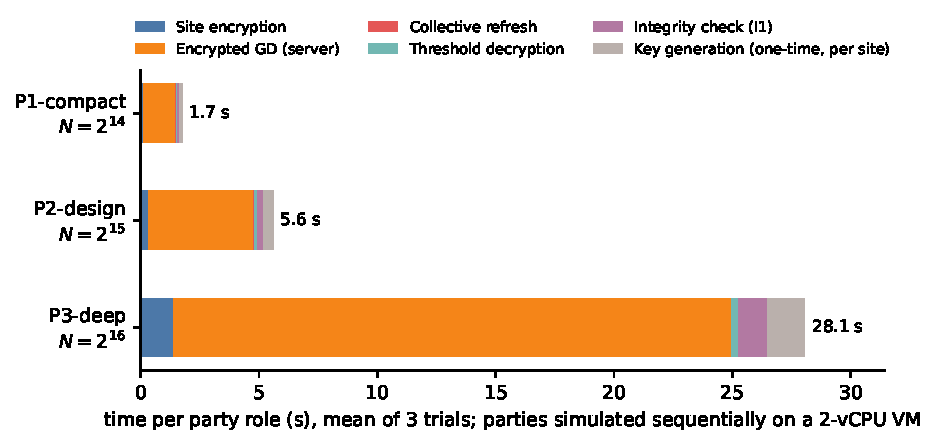
\includegraphics[width=0.94\textwidth]{time_breakdown.pdf}
\caption{Time per role. Encrypted gradient descent dominates every set; refreshes and threshold decryption are each under 3\% of the total.}
\label{fig:time}
\end{figure}

\begin{table}[H]
\centering\small
\caption{Time (seconds, mean $\pm$ sd over 3 trials) against the Part~2 budget for P2. Baseline: numpy, 3.4~ms.}\label{tab:time}
\begin{tabularx}{\textwidth}{@{}lRRRr@{}}
\toprule
\textbf{Operation} & \textbf{P1-compact} & \textbf{P2-design} & \textbf{P3-deep} & \textbf{Part 2 budget} \\
\midrule
Key generation, per site (one-time) & $0.12\pm0.01$ & $0.40\pm0.01$ & $1.57\pm0.06$ & $\le 30$ \\
Encryption, per site (10 ciphertexts) & $0.10\pm0.00$ & $0.34\pm0.02$ & $1.41\pm0.10$ & $\le 5$ \\
One GD iteration (8 products, 7 rotations) & $0.053\pm0.002$ & $0.170\pm0.005$ & $0.91\pm0.05$ & $\le 3$ \\
All GD iterations (26 products) & $1.37\pm0.06$ & $4.43\pm0.13$ & $23.5\pm1.4$ & $\le 80$ \\
One collective refresh & 0.012 & 0.035 & -- & $\le 10$ \\
Threshold decryption (share + fusion) & $0.020\pm0.004$ & $0.057\pm0.008$ & $0.061\pm0.005$ & $\le 2$ \\
I1 integrity hashing (site + server) & 0.074 & 0.261 & 1.24 & -- \\
\textbf{Online latency, Mode B} & $\mathbf{1.66\pm0.08}$ & $\mathbf{5.19\pm0.11}$ & $\mathbf{26.3\pm1.6}$ & $\le 120$ \\
Slowdown vs non-private baseline & 490$\times$ & 1{,}530$\times$ & 7{,}760$\times$ & -- \\
Peak memory (whole simulation) & 0.36 GB & 1.32 GB & 3.86 GB & $\le 4$ GB \\
\bottomrule
\end{tabularx}
\end{table}

\begin{table}[H]
\centering\small
\caption{Measured sizes (MB) of objects that cross the network, against the Part~2 budget for P2.}\label{tab:size}
\begin{tabularx}{\textwidth}{@{}lRRRr@{}}
\toprule
\textbf{Object} & \textbf{P1-compact} & \textbf{P2-design} & \textbf{P3-deep} & \textbf{Part 2 budget} \\
\midrule
Fresh ciphertext & 1.57 & 5.77 & 30.4 & 4.6 \\
Relinearization key / each rotation key & 6.29 & 23.6 & 151 & 19.7 \\
Upload per site, key generation (once) & 58.2 & 218 & 785 & $\le 180$ \\
Upload per site, regression inputs (9 ct) & 14.2 & 51.9 & 274 & 46 \\
Refresh share, per site per refresh & 1.18 & 3.67 & -- & $\le 2$ \\
Partial decryption share & 0.53 & 2.36 & 1.58 & $\le 0.5$ \\
Server key storage & 50.3 & 189 & 604 & 160 \\
\bottomrule
\end{tabularx}
\end{table}

\textbf{Against the Part~2 budget.} Every time budget is met with a 10--500$\times$ margin. Five size budgets are exceeded. Part~2 estimated sizes from $\log Q$ bits, but OpenFHE stores each RNS limb in a 64-bit word: 11 limbs $\times$ 2 polynomials $\times$ $2^{15}$ coefficients $\times$ 8 bytes is exactly the measured 5.77~MB, 26\% above the estimate. Decryption shares are larger than budgeted because the final ciphertext still has 9 of its 11 limbs. Reducing it to the last level before decryption would shrink shares about 9$\times$. Key-generation upload is 21\% over budget, but the ablation below brings it under.

\textbf{Non-private baseline.} The plaintext pipeline takes 3.4~ms and gives the exact OLS answer. The private version is about 1{,}500$\times$ slower on P2 and, at $K=27$, 2.7\% less accurate. Doubling to $K=54$ closes the accuracy gap to 0.07\% for 4~s more server time.

\begin{figure}[H]
\centering
\begin{minipage}[t]{0.49\textwidth}\centering
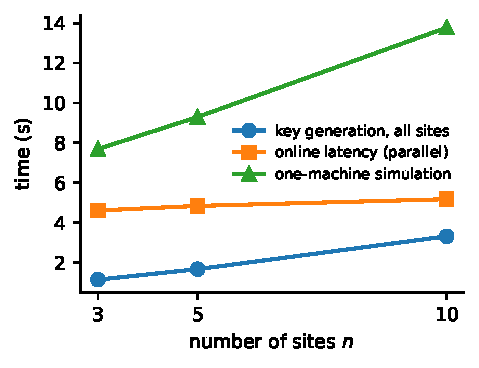
\includegraphics[width=\textwidth]{scaling.pdf}
\caption{P2 with $n=3,5,10$ sites. Online latency stays flat (4.6 to 5.2~s); key generation grows linearly (1.1 to 3.3~s total).}\label{fig:scale}
\end{minipage}\hfill
\begin{minipage}[t]{0.49\textwidth}\centering
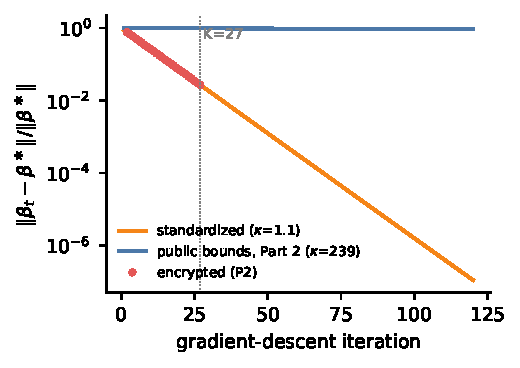
\includegraphics[width=\textwidth]{convergence.pdf}
\caption{Convergence to OLS. The Part~2 scaling stalls; standardized GD converges linearly, and encrypted iterates (dots) track it.}\label{fig:conv}
\end{minipage}
\end{figure}

\textbf{Scaling with sites.} Per-site cost does not depend on $n$: 0.33--0.38~s for key generation and 218~MB of upload. The server's per-iteration work is independent of $n$, so online latency rises only 12\% from 3 to 10 sites, which is the cost of more refresh and decryption shares. Coefficient error stays below $10^{-6}$ with 10 flooded shares.

\textbf{Ablations (P2).} Hoisted rotations~[10], which share one key-switching decomposition across the 7 rotations of $\beta$, cut iteration time from 0.211~s to 0.176~s (17\%). Generating rotation keys only for shifts $\{1,2,4\}$ and composing the rest costs 5\% per iteration (0.184~s). In exchange it cuts rotation-key material from 165~MB to 71~MB, per-site key upload from 218~MB to 124~MB (now under budget) and peak memory from 1.32 to 0.72~GB. That is what made P3 fit in 7~GB.

\section{Convergence and the Part 2 Design}\label{sec:conv}

Part~2 scaled features to $[0,1]$ with public bounds and divided by the public record bound $N_b$, so that no pooled statistic is needed before regression. On this cohort that makes $\tilde G$ badly conditioned: condition number $\kappa=239$, $\lambda_{\min}=0.0019$. With the provably safe step $\eta=1/d$, the contraction factor $1-\eta\lambda_{\min}$ is about 0.9998. Figure~\ref{fig:conv} shows the result: the relative coefficient error is 97.3\% after 27 iterations, 96.0\% after 54, and still 93.3\% after 120. The encrypted run on P2 reproduces 97.25\% exactly, so the failure lies in the algorithm, not the encryption. Standardizing with pooled means and standard deviations brings $\kappa$ to 1.12 and the error to 2.7\% at $K=27$ and 0.07\% at $K=54$. Prediction quality hides this problem: the unconverged model's mean squared error is only 6.6\% above OLS, because readmission is mostly unexplained noise. That is why coefficient error, not prediction error, is the metric reported here.

\section{Limitations and Discussion}\label{sec:lim}

\textbf{1. Semi-honest only; I1 checks inputs, not computation.} I1 stops a server from dropping, duplicating or substituting inputs. It does not stop a malicious server from evaluating a \emph{different function} on the right inputs and obtaining its decryption, for example one site's ciphertext alone. Because the server's whole computation takes about 5~s and is deterministic given its transcript, a practical fix is \emph{replicated verification}: each site re-runs the evaluation and decrypts only if its output hash matches the server's. Malicious sites (out-of-range inputs) would need the ZK range proofs (I2) left as design-only in Part~2.

\textbf{2. Flooding is fixed, not calibrated to a query budget.} The IND-CPA$^D$ defense~[5,6] needs flooding noise sized to the statistical security parameter and the number of decryptions. OpenFHE's threshold CKKS uses a fixed $\sigma=2^{20}$ instead. My contribution here is procedural: rescale before decrypting, so that the flood exceeds the ciphertext's own noise. The margin is not formally quantified. Calibrated flooding would lower precision further, and P1's 11.8 bits leave no room for it, so P2's 20.7 bits is the minimum I would deploy. The query budget $Q_{\max}=32$ from Part~2 is not enforced in code.

\textbf{3. The fix for convergence costs privacy.} The standardization round releases 14 statistics that Part~2's Mode~B kept secret. Alternatives would be encrypted preconditioning (one more level per iteration) or Mode~A-only output. Neither was evaluated.

\textbf{4. Leakage that cryptography cannot remove.} With $n=3$, two colluding sites can subtract their own moments from the released aggregates. Differential privacy noise was not implemented.

\textbf{5. Simulation, not deployment.} All parties run in one process without TLS or network delay, so the reported latency is compute only. At 100~Mb/s, P2's per-site uploads (218~MB of keys once, then 52~MB of inputs per study) would add about 17~s and 4~s; transfer would then match compute. Timings come from one 2-vCPU VM with OpenMP enabled, so absolute numbers are machine-specific; the ratios between sets are the robust result.

\textbf{6. Scope of the model and data.} A linear probability model is fitted to a binary outcome. Logistic regression needs a polynomial sigmoid, which is deeper (P3 shows that depth costs 5$\times$). The data are synthetic with weakly correlated features, so $\kappa\approx1$ after standardization. Real clinical features are more correlated and would need more iterations, which is affordable because each refresh costs about 35~ms. Rounding releases to 4 significant digits is not justified on P1, whose error ($2.8\times10^{-4}$) is about 1.4\% of the smallest coefficients.

\textbf{Conclusion.} Threshold CKKS makes multi-site regression practical at a 128-bit security level: about 5~s of compute and 20.7 bits of precision on P2, with every key share required to decrypt. The evaluation also showed where the paper design needed changes: conditioning, refresh headroom and the gap between fixed and calibrated flooding. These are exactly the issues a deployment would need to address.

\section*{References}
\footnotesize
\begin{enumerate}[label={[\arabic*]},leftmargin=*,itemsep=1pt]
\item Jung Hee Cheon, Andrey Kim, Miran Kim, and Yongsoo Song. 2017. Homomorphic encryption for arithmetic of approximate numbers. In \emph{ASIACRYPT 2017} (LNCS, Vol. 10624). Springer, 409--437. \url{https://doi.org/10.1007/978-3-319-70694-8_15}
\item Jung Hee Cheon, Kyoohyung Han, Andrey Kim, Miran Kim, and Yongsoo Song. 2019. A full RNS variant of approximate homomorphic encryption. In \emph{SAC 2018} (LNCS, Vol. 11349). Springer, 347--368. \url{https://doi.org/10.1007/978-3-030-10970-7_16}
\item Gilad Asharov, Abhishek Jain, Adriana L\'opez-Alt, Eran Tromer, Vinod Vaikuntanathan, and Daniel Wichs. 2012. Multiparty computation with low communication, computation and interaction via threshold FHE. In \emph{EUROCRYPT 2012} (LNCS, Vol. 7237). Springer, 483--501. \url{https://doi.org/10.1007/978-3-642-29011-4_29}
\item Christian Mouchet, Juan Troncoso-Pastoriza, Jean-Philippe Bossuat, and Jean-Pierre Hubaux. 2021. Multiparty homomorphic encryption from ring-learning-with-errors. \emph{Proceedings on Privacy Enhancing Technologies} 2021, 4, 291--311. \url{https://doi.org/10.2478/popets-2021-0071}
\item Baiyu Li and Daniele Micciancio. 2021. On the security of homomorphic encryption on approximate numbers. In \emph{EUROCRYPT 2021} (LNCS, Vol. 12696). Springer, 648--677. \url{https://doi.org/10.1007/978-3-030-77870-5_23}
\item Baiyu Li, Daniele Micciancio, Mark Schultz, and Jessica Sorrell. 2022. Securing approximate homomorphic encryption using differential privacy. In \emph{CRYPTO 2022} (LNCS, Vol. 13507). Springer, 560--589. \url{https://doi.org/10.1007/978-3-031-15802-5_20}
\item Martin Albrecht et al. 2021. Homomorphic encryption standard. In \emph{Protecting Privacy through Homomorphic Encryption}. Springer, 31--62. \url{https://doi.org/10.1007/978-3-030-77287-1_2}
\item Shai Halevi and Victor Shoup. 2014. Algorithms in HElib. In \emph{CRYPTO 2014} (LNCS, Vol. 8616). Springer, 554--571. \url{https://doi.org/10.1007/978-3-662-44371-2_31}
\item Ahmad Al Badawi, Jack Bates, Flavio Bergamaschi, et al. 2022. OpenFHE: Open-source fully homomorphic encryption library. In \emph{Proceedings of the 10th Workshop on Encrypted Computing \& Applied Homomorphic Cryptography (WAHC '22)}. ACM, 53--63. \url{https://doi.org/10.1145/3560827.3563379}
\item Shai Halevi and Victor Shoup. 2018. Faster homomorphic linear transformations in HElib. In \emph{CRYPTO 2018} (LNCS, Vol. 10991). Springer, 93--120. \url{https://doi.org/10.1007/978-3-319-96884-1_4}
\end{enumerate}

\end{document}
